\documentclass[11pt,a4paper,openany]{article}
\usepackage{amsmath}             %%%%多种的公式环境和数学命令
\usepackage{amssymb}             %%%%数学符号生成命令
\usepackage{array}               %%%%数组和表格
\usepackage{booktabs}            %%%%水平的表格线
\usepackage{bm}
\usepackage{calc}                %%%%四则运算
\usepackage{caption}             %%%%插图和表格
% \usepackage{ctex}                %%%%中文字体
% \usepackage{ctexcap}             %%%%中文字体和标题
\usepackage{fancyhdr}            %%%%页眉页脚设置
% \usepackage{floatrow}
\usepackage{graphicx}            %%%%插图
\usepackage{geometry}            %%%%版面尺寸控制
\geometry{left=2cm, right=2cm, top=2cm, bottom=2cm, head=2cm, foot=1cm}
% head=?cm, headmap=?cm
\usepackage{hyperref}            %%%%超链接
\usepackage{ifthen}              %%%%条件
\usepackage{longtable}           %%%%跨页表格
\usepackage{multicol}            %%%%多栏
\usepackage{ntheorem}            %%%%定理设置
\usepackage{paralist}            %%%%列表
\usepackage{subfigure}
\usepackage{tabularx}            %%%%表格的列宽
\usepackage{titlesec}            %%%%章节标题
\usepackage{fancyvrb}            %%%%抄录
\usepackage{fontspec}            %%%%字体
\usepackage{titletoc}            %%%%目录格式
\usepackage{xcolor}              %%%%颜色处理
\usepackage{xeCJK}               %%%%中日朝文字处理

\begin{document}
\title{Omega and Phi production in a multiphase transport model with enhanced local parton density fluctuation scenario}
\date{2017/08/15}
\maketitle

\begin{abstract}
  Searching for QCD critical point and mapping the QCD phase diagram are major science goals of the
  Beam Energy Scan program in Heavy-Ion Collisions. Many exciting results have been published in the
  past decades and deepen our understanding on the QCD phase transition, such as the non-monotonic of
  net-proton direct flow, the net-baryon kurtosis. On the other hand, multi-strange hadron such as
  Omega and Phi are important probes for the search of the QCD phase boundaries. The Omega and Phi
  are expected to have relatively small hadronic interaction cross sections. Therefore, they can
  carry the information directly from the chemical freeze-out stage with little or no distortion due
  to hadronic rescattering. As a result, the production of the Omega and Phi particle offers a unique
  advantage in probing the transition from partonic to hadronic dynamics.  In this talk, we study the
  Omega and Phi production in a multiphase transport model with employment enhanced local parton
  density fluctuation scenario. Our calculations describe the $p_{T}$ spectrum of experiment data
  well and predict an enhanced production of Omega and Phi near the QCD phase boundary. In
  particularly, we find that the Baryon/Meson ratio is more sensitive to the local density
  fluctuation strength. The ratio will increased significantly in comparison with original AMPT
  model calculation. We also study the flow harmonic of multistrange hadron in response to the local
  density fluctuation.
\end{abstract}

\section{INTRODUCTION}
Lattice quantum chromodynamics(QCD) calculations suggest that at high temperature and low baryon
chemical potential($\mu_{B}$), there will be a phase transition from the hadron gas to the quark
gluon plasma(QGP), and the phase transition is smooth and continuous. Heavy ion collisions at
relativistic energy provide a possibility to study the properties of QGP and QCD phase diagram.
The production of multi-strange particles provides a way to investigate the properties of QCD phase
diagram. The strange quarks are create

\section{AMPT MODEL}
The multiphase transport (AMPT) model is a hybrid model to describe heavy ions collisions at
relativistic energies~\cite{AMPT-MODEL}, it has two versions: default version and string melting
version, for our study, we adopt the string melting version. The AMPT model consists of four
components. The initial stage is described by heavy ion jet interaction generator (HIJING)
model~\cite{HIJING} that is designed to simulate multiple jets and particle production in heavy ion
collisions. Zhang's parton cascade (ZPC)~\cite{ZPC} is used to describe scattering among partons,
until now, it only includes two-body interaction, but we think it is enough to describe interaction
between partons. The hadronization of parton is based on a simple quark coalescence
model~\cite{AMPT-MODEL}. The scattering of resulting hadrons is described by a relativistic
transport (ART) model~\cite{ART,ART2}. In AMPT, for the string melting version, all excited strings
are converted to partons. In the transport approach, interactions among partons are described by
equations of their Wigner distortion functions, which describe semicalssically their density
distortions in phase space~\cite{ZPC}. the scattering of parton can be described use the following equation in
ZPC
\begin{equation}
  \label{eq:1}
  \sigma_{gg} \approx \frac{9\pi\alpha_{s}^{2}}{2\mu^{2}}
\end{equation}
where $\alpha_{s}$ is the strong coupling constant, and $\mu$ is the screening mass which depend on
the medium effect~\cite{ZPC}. For the AMPT program that is currently in use, it does not contain QCD
fluctuation. However, according to the calculation of lattice QCD, the phase transition is smooth
and continuous between hadron gas and QGP, this implies that there may be a critical point at the
end of the first order phase transition line. Viewed from the thermodynamic, a critical point is a
point at which a single thermodynamic state bifurcates into two macroscopically distinct states.
This bifurcation may leads to long-ranged thermal fluctuations. To model this effect, a large
density fluctuation is introduced at the end of scattering of parton. Shown in Fig.~1 is the
distributions of parton in the transverse plane.
\begin{figure}[!ht]
  \centering
  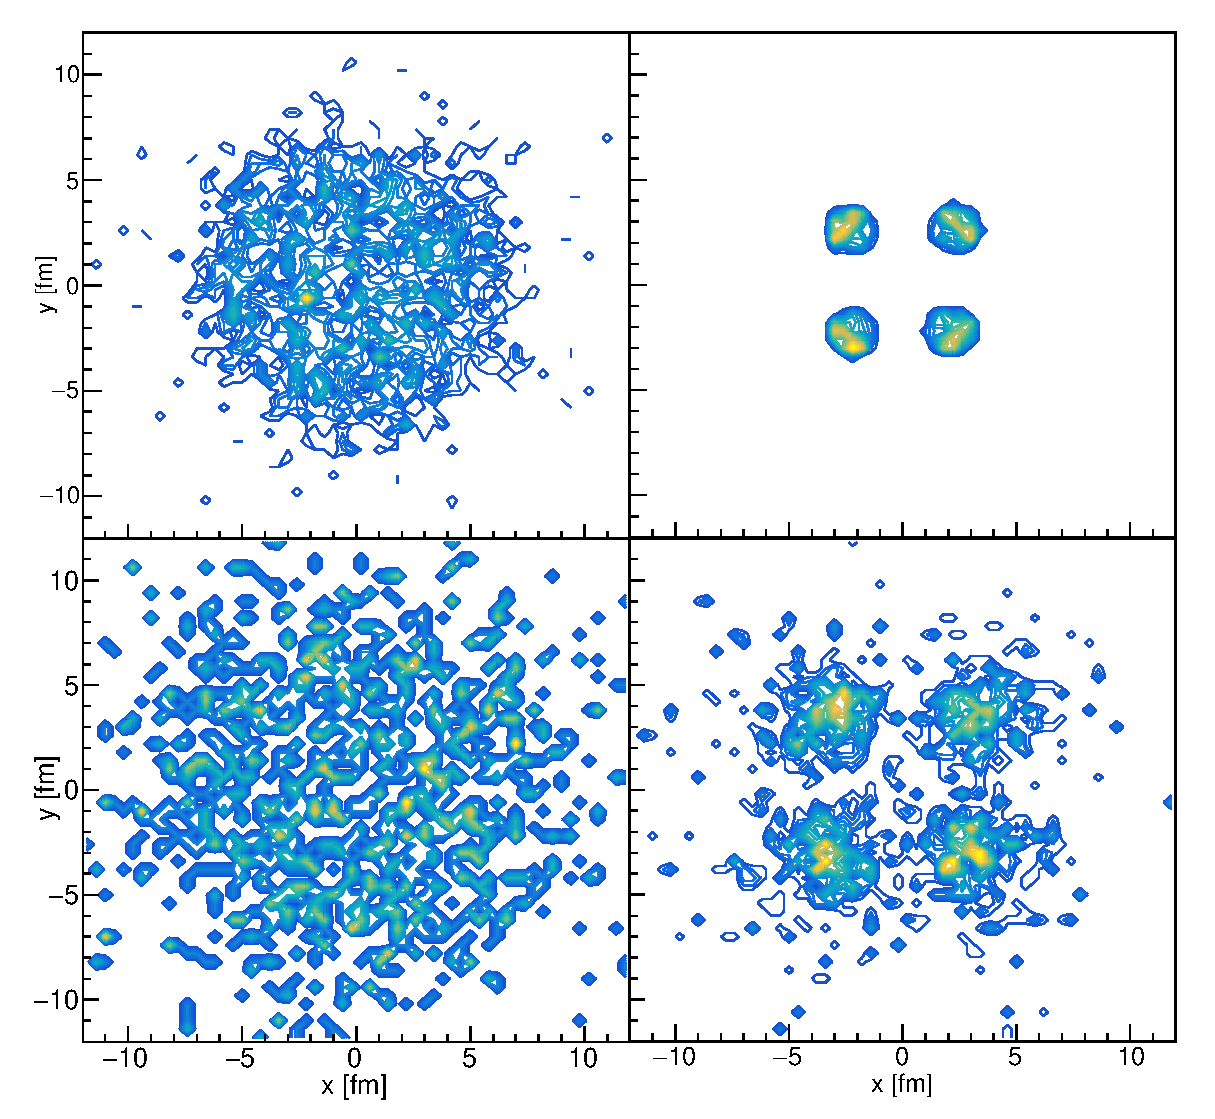
\includegraphics[width=0.5\textwidth]{./figure/square.eps}
  \caption{The distributions of parton in the transverse plane. Left figure: The distribution of
           parton that does not include the QCD fluctuation. Right figure: The distribution of
           parton that takes into account QCD fluctuation.}
  \label{fig:phaseSpace}
\end{figure}
From coalescence picture, the fluctuation of parton can be served in hadronic matter.

\section{QUARK WIGNER PHASE-SPACE FUNCTIONS OF $\Phi$ AND $\Omega$}
A dynamical coalescence model has been used to study the production of $\Omega$ and $\phi$,
according to this model, the probability for producing a hadron from partons is given by the
overlap of parton phase-space distributions with the parton Wigner phase-space function inside
hadron~\cite{COALESCENCE}. The multiplicity of a $M$-parton hardon in a heavy-ion collision is
given by
\begin{equation}
  \label{eq:2}
  N_{M} = G  \int{}d\bm{r}_{i_{1}}\,d\bm{q}_{i_{1}}\dots{}d\bm{r}_{i_{M-1}}\,d\bm{q}_{i_{M-1}}\times{}\langle{}\sum_{i_{1}>i_{2}>\dots>i_{M}}\rho_{i}^{W}(\bm{r}_{i_{1}},\,\bm{q}_{i_{1}}\dots{}\bm{r}_{i_{M-1}},\,\bm{q}_{i_{M-1}}) \rangle{}
\end{equation}
In Eq.~(\ref{eq:2}), $\langle{}$\dots$\rangle{}$ represents the event averaging; $\textbf{r}_{i_{1}}$,\dots{},$\textbf{r}_{i_{M-1}}$ and
$\textbf{q}_{i_{1}}$,\dots,$\textbf{q}_{i_{M-1}}$ are the $M-1$ relative coordinates and momenta
in the $M$-parton rest frame; $\rho_{i}^{W}$ is the Wigner phase-space function inside the hadron
and G is the statistical factor for the $M$ partons.
\par
To determine the quark Wigner phase-space functions inside $\Omega$ and $\phi$, we need quark
wave functions. The quark wave functions can be token as a spherical harmonic
oscillator~\cite{waveFunction}. For the $\phi$ particle, it can be expressed as
\begin{equation}
  \label{eq:3}
  \psi(\bm{r}_{1},\,\bm{r}_{2}) = 1 / (\pi\sigma_{\phi}^{2})^{3/4}\;exp\left[-r^{2}/(2\sigma_{\phi}^{2})\right].
\end{equation}
where $\sigma_{\phi}$ is a size parameter of $\phi$, its normalized wave function leads to a root
mean-square radius $R_{\phi} = (3/8)^{1/2}\sigma_{\phi}$. The quark Wigner function in $\phi$
particle can be expressed as
\begin{equation}
  \label{eq:4}
  \rho_{\phi}^{W} = 8 exp\left(-\frac{r^2}{\sigma_{\phi}^2}-\sigma_{\phi}^{2}k^{2}\right).
\end{equation}
where \textbf{k} = ($\textbf{k}_{1}-\textbf{k}_{2})/2$ is the relative distance between s and
$\bar{s}$.
\par
Similarly, for $\Omega^{-}$ and $\bar{\Omega}^{+}$ particles, their wave function can be described
by the following equation
\begin{equation}
  \label{eq:5}
  \psi(\bm{r}_{1},\bm{r}_{2},\bm{r}_{3}) = (3\pi^{2}\sigma_{\Omega}^{4})^{-3/4}\,exp\left(-\frac{\rho^2+\lambda^2}{2\sigma_{\Omega}^{2}}\right).
\end{equation}
The quark Wigner phase-space function inside the $\Omega^{-}$ and $\bar{\Omega}^{+}$ baryon can be
expressed as
\begin{equation}
  \label{eq:6}
  \rho_{\Omega}^{W}(\rho, \lambda, \bm{k}_{\rho}, \bm{k}_{\lambda}) = 64\;exp\left(-\frac{\rho^2+\lambda^2}{\sigma_{\Omega}^{2}}\right)\;exp\left[-(\bm{k}_{\rho}^{2}+\bm{k}_{\lambda}^{2})\sigma_{\Omega}^{2}\right]
\end{equation}
where $\rho$ and $\lambda$ are relative coordinates of quark, $\textbf{k}_\rho$ and
$\textbf{k}_\lambda$ are relative momenta, $\sigma_{\Omega}$ is a size parameter that is related
to the root mean-square radius $R_{\Omega}$.
\par
The two parameters $\sigma_{\phi}$ and $\sigma_{\Omega}$ in the quark Wigner phasespace functions
inside the $\phi$ meson and $\Omega$ baryon are related to their root-mean-square (RMS) radius. we
take their values of RMS as $R_{\phi} = 0.65$ fm and $R_{\Omega} = 1.2$ fm~\cite{COALESCENCE}.




\section{RESULT}
Using the parton phase-space information and dynamical coalescence method, we study the effect
of QCD fluctuation on transverse-momentum spectra of $\phi$ and $\Omega$ as well as their flow.
\begin{figure}[!h]
  \begin{minipage}{0.5\textwidth}
    \centering
    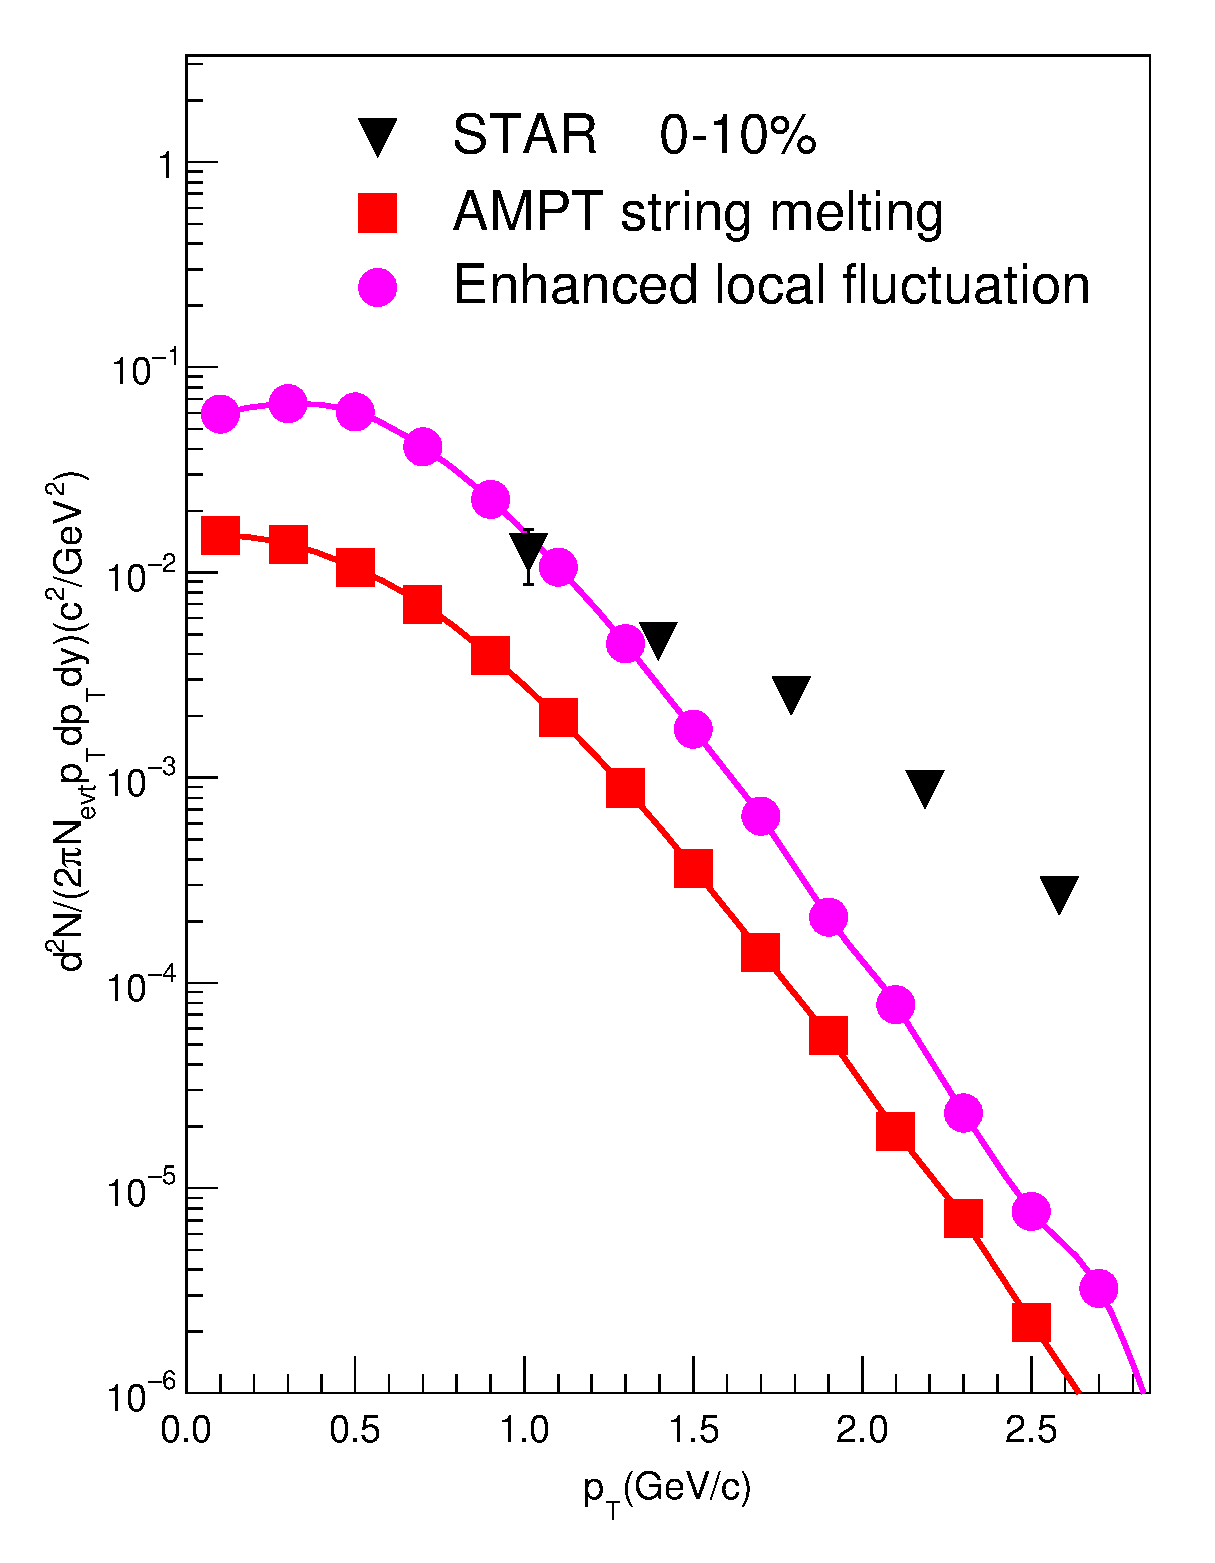
\includegraphics[width=2.5in]{./figure/omegaYield.eps}
    \caption{Transverse momentum spectra of $\Omega$ from the string melting AMPT and enhanced local
fluctuation AMPT for centrality (0-10\%) Au+Au collisions at 11.5 GeV.}
    \label{fig:omegaspectra}
  \end{minipage}
  \begin{minipage}{0.5\textwidth}
    \centering
    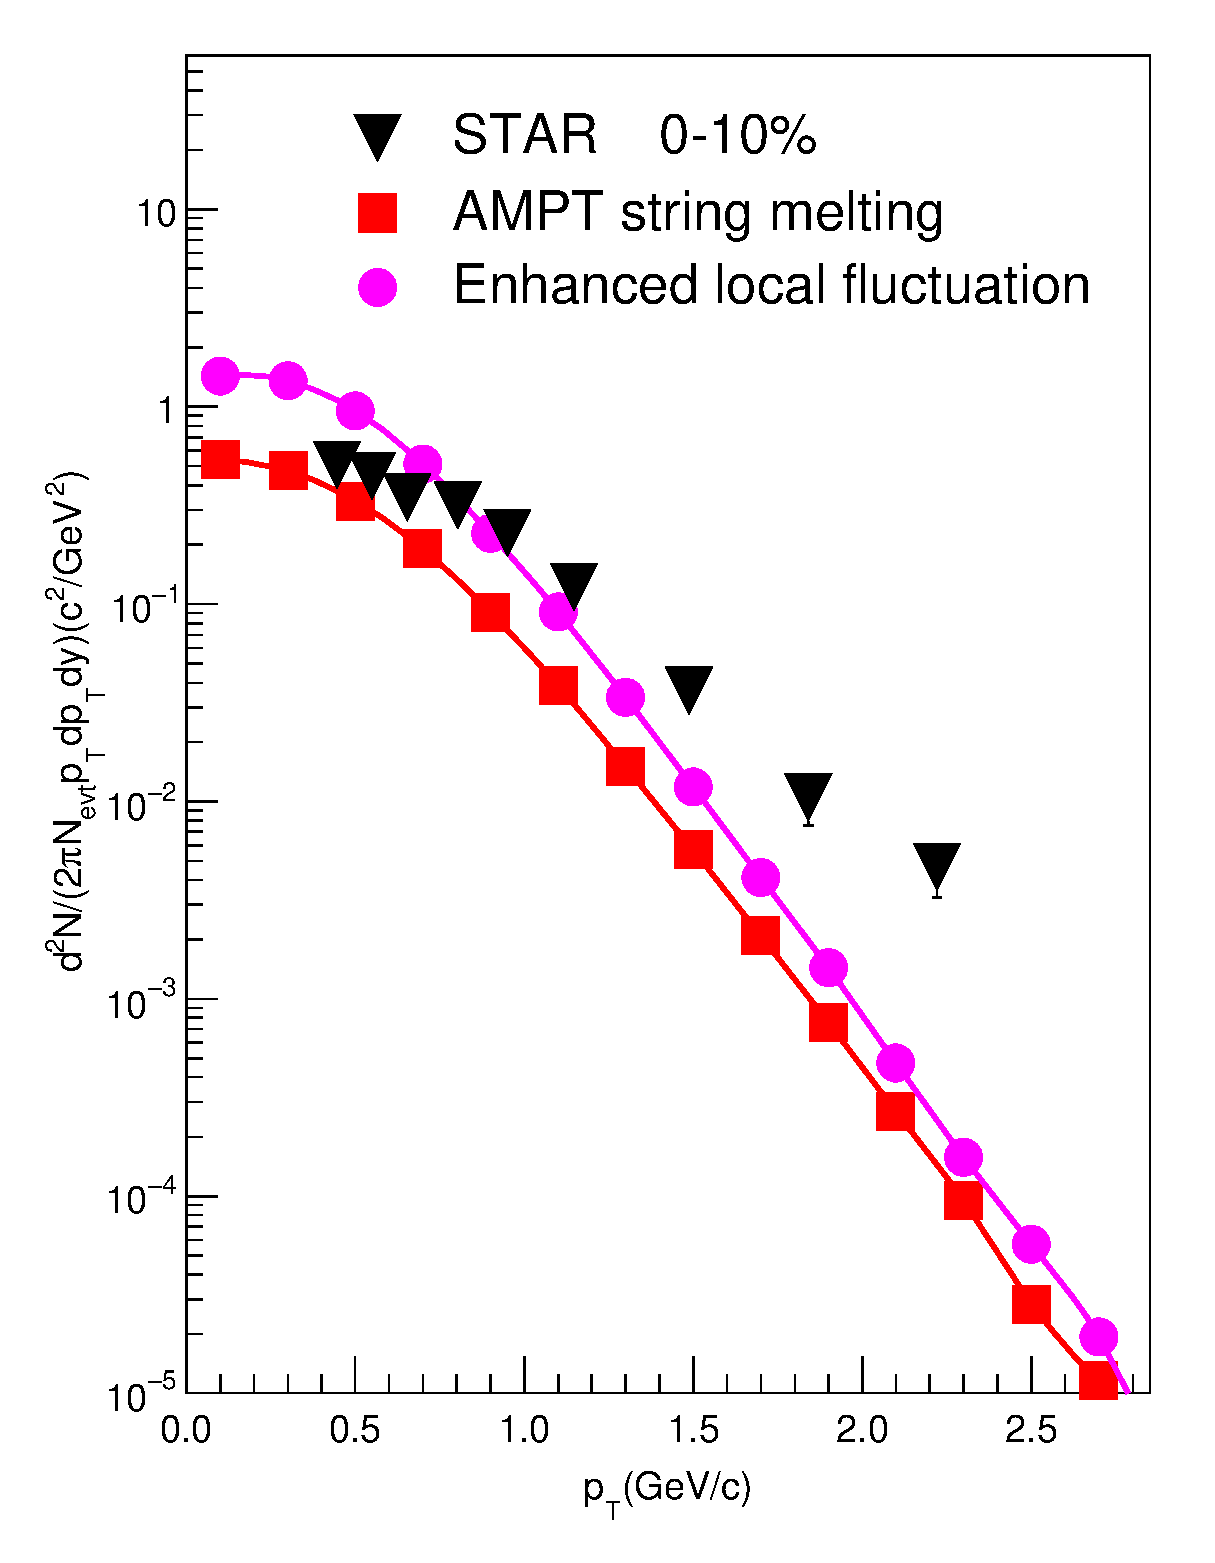
\includegraphics[width=2.5in]{./figure/phiYield.eps}
    \caption{Transverse momentum spectra of $\phi$ from the string melting AMPT and enhanced local
fluctuation AMPT for centrality (0-10\%) Au+Au collisions at 11.5 GeV.}
    \label{fig:phispectra}
  \end{minipage}
\end{figure}
In Fig. \ref{fig:omegaspectra} and Fig. \ref{fig:phispectra}, we present the transverse momentum
distributions of $\Omega$ and $\phi$
measured at midrapidity. From these two figures, it is obvious that the QCD fluctuation has the
trend to increase the transverse momentum spectra of $\Omega$ and $\phi$. However, in AMPT, the
total number of strange quarks follows the same distribution in different events, in other words,
through dynamical coalescence method, the total number of
\textquotedblleft{strange}\textquotedblright hadron times the valence quarks number should satisfy
the same distribution. So the transverse momentum spectra can not directly response the QCD
fluctuation.
\par
Therefore, we also study the ratio of $\Omega/\phi$ as a function of $p_t$. The result is presented
in Fig. \ref{fig:ratio}, 
\begin{figure}[!h]
  \centering
  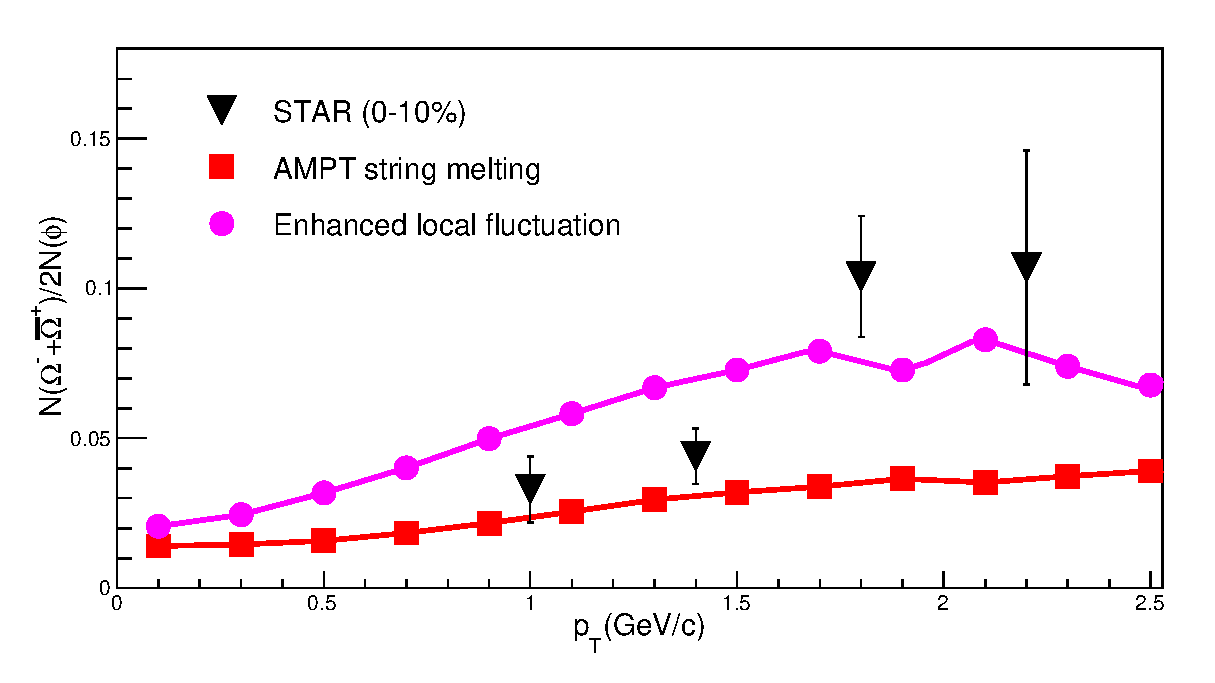
\includegraphics[width=0.8\textwidth]{./figure/Ratio.eps}
  \caption{Ratio}
  \label{fig:ratio}
\end{figure}
The measured $N(\Omega^{-}+\bar{\Omega}^{+})/2N(\phi)$ ratio from string melting  AMPT is flat and 
can describe the experiment data in low $p_t$, but it underestimates the ratio in high $p_{t}$. For 
the enhanced local fluctuation result, it is obvious that QCD fluctuation has the trend to increase
the ratio of $\Omega$ to $\phi$.

\section{Anisotropic flows of $\phi$ and $\Omega$}
The collectivity in high-energy heavy-ion collisions can be measured through final particle 
azimuthal anisotropy. The anisotropy coefficients are generally obtained from Fourier expansion
of final particle azimuthal distortion~\cite{malong}. i.e.,
\begin{equation}
  \label{eq:7}
  E\frac{d^{3}N}{d^{3}p} = \frac{1}{2\pi}\frac{d^{2}N}{p_{T}dp_{t}dy}\left(1+\sum^{N}_{i=1}{2v_{n}cos[n(\phi-\psi_{RP})]}\right).
\end{equation}
where $E$ is the energy of final particle, $p_{T}$ is the transverse momentum, y is the rapidity, 
$\phi$ is the azimuthal angle of particle and $\psi_{RP}$ is the reaction plane angle. The Fourier 
coefficients $v_{n}(n=1,2,\dots)$ can be described by the following equation
\begin{equation}
  \label{eq:8}
  v_{n} = \langle{cos(n[\phi-\psi_{RP}])}\rangle.
\end{equation}
Similarly, the calculation of harmonic flow $v_{n}$ can be relative to the participant plane angle
$\psi_{n}\{P\}$. For the study of QCD fluctuation, we think this method is more appropriate. The
participant plane angle can be defined by the following equation
\begin{equation}
  \label{eq:9}
  \psi_{n}\{P\} = \frac{1}{n}\left[arctan\frac{\langle{r^{2}sin(n\varphi)}\rangle}{\langle{r^{2}cos(n\varphi)}\rangle}+\pi\right].
\end{equation}
where $n$ is $n$th-order participant plane, $r$ and $\varphi$ are the coordinates position and 
azimuthal angle of parton, the symbol $\langle{\dots}\rangle$ represents density weighting.
\begin{figure}[!ht]
  \begin{minipage}{0.5\textwidth}
    \centering
    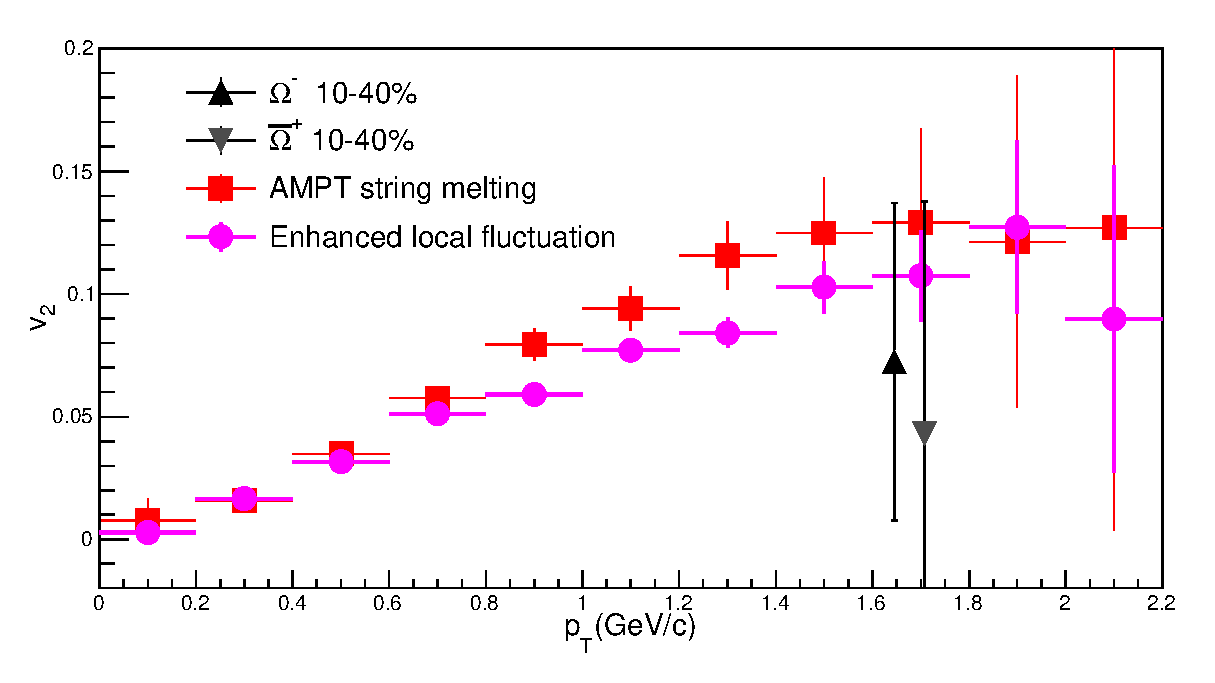
\includegraphics[width=2.5in]{./figure/omegaFlow.eps}
    \caption{Transverse momentum spectra of $\Omega$ from the string melting AMPT and enhanced local
fluctuation AMPT for centrality (0-10\%) Au+Au collisions at 11.5 GeV.}
    \label{fig:omegaflow}
  \end{minipage}
  \begin{minipage}{0.5\textwidth}
    \centering
    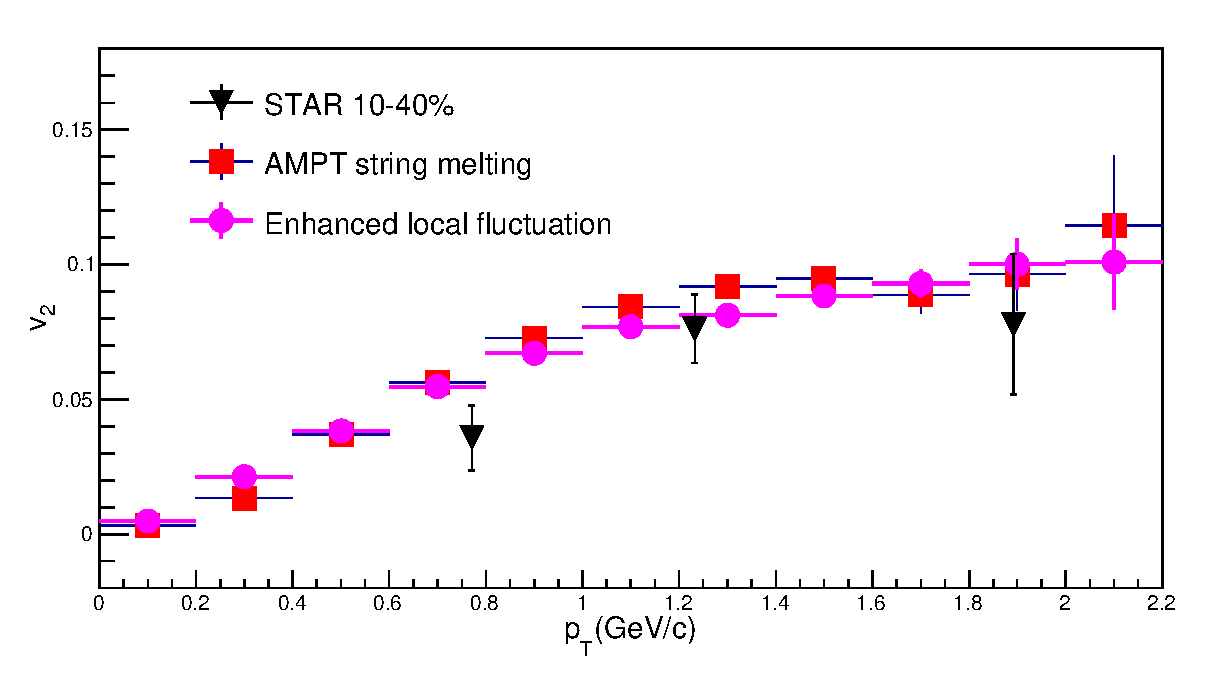
\includegraphics[width=2.5in]{./figure/phiFlow.eps}
    \caption{Transverse momentum spectra of $\phi$ from the string melting AMPT and enhanced local
fluctuation AMPT for centrality (0-10\%) Au+Au collisions at 11.5 GeV.}
    \label{fig:phiflow}
  \end{minipage}
\end{figure}
In Fig. \ref{fig:omegaflow} and \ref{fig:phiflow}, we show the results of $\Omega$ and $\phi$ 
$v_{2}$. In  the range of experiment error, the data from string melting AMPT and enhanced local 
fluctuation AMPT can be consistent with the experiment. Comparing the two sets of AMPT model data, 
the size of  $v_{2}$ is almost same. because, In AMPT model, the $v_{2}$ is mainly developed in the 
parton cascade stage, moreover, the $v_{2}$ of $\Omega$ and $\phi$ is not affected by the hadron 
interaction due to its small cross-section. 

\section{Summary}
Based on the parton phase-space information and dynamical coalescence method, we study the effect
of QCD fluctuation on the production of $\Omega$ baryon and $\phi$ meson. we have calculated the
transverse momentum spectra, ratio and elliptic flow of these particles. For the production of 
$\Omega$ and $\phi$, we have found that the QCD fluctuation have the trend to increase the ratio
of baryon-to-meson, it can be used as a valid evidence for detecting the QCD critical point.
For the $v_{2}$ of $\Omega$ and $\phi$, we have found that it is not sensitive to the QCD 
fluctuation.


\begin{thebibliography}{88}
\bibitem{AMPT-MODEL} Z. W. Lin, C. M. Ko, B. A. Li, B. Zhang and S. Pal, Phys. Rev. C {\bf 72},
 064901 (2005).
\bibitem{HIJING} X. N. Wang and M. Gyulassy, Phys. Rev. D \textbf{44}, 3501 (1991); M. Gyulassy and
X. N. Wang, Comput. Phys. Commun. \textbf{83}, 307 (1994).
\bibitem{ZPC} B. Zhang, Comput. Phys. Commun. \textbf{109}, 193 (1998).
\bibitem{ART} B. A. Li and C. M. Ko, Phys. Rev. C \textbf{52}, 2037 (1995).
\bibitem{ART2} B. A. Li, A. T. Sustich, B. Zhang, and C. M. Ko, Int. J. Mod. Phys. E \textbf{10},
267 (2001).
\bibitem{COALESCENCE} L. W. Chen and C. M. Ko, Phys. Rev. C \textbf{73}, 044903 (2006).
\bibitem{waveFunction} L. w. Chen, C. M. Ko and B. A. Li, Nucl. Phys. A \textbf{757}, 809 (2003).
\bibitem{malong} L. Ma, G. L. Ma and Y. G. Ma, Phys. Rev. C \textbf{89}, 044907 (2014)
\end{thebibliography}

\end{document}

%%% Local Variables:
%%% mode: latex
%%% TeX-master: t
%%% End:
